\begin{figure}[ht!]
\centering
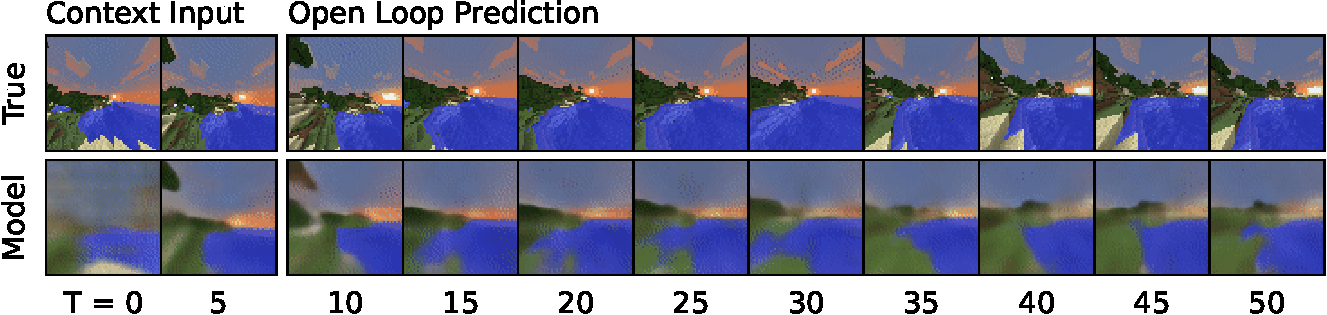
\includegraphics[width=\linewidth,trim={0 .5cm 0 0},clip]{openl/mine1} \\[1ex]
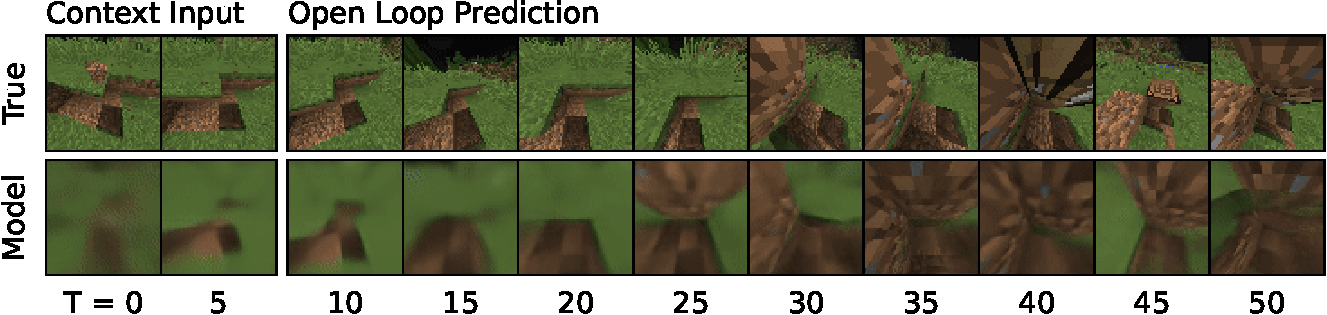
\includegraphics[width=\linewidth,trim={0 .5cm 0 .5cm},clip]{openl/mine2} \\[1ex]
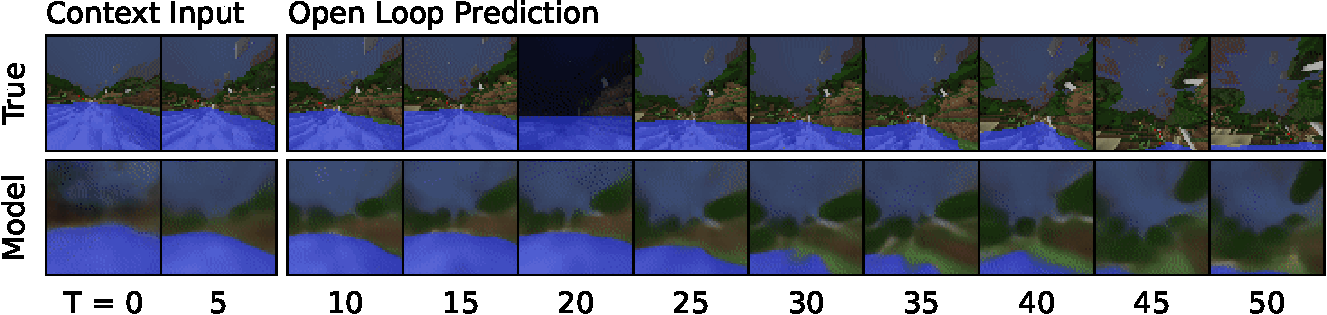
\includegraphics[width=\linewidth,trim={0 .5cm 0 .5cm},clip]{openl/mine3} \\[1ex]
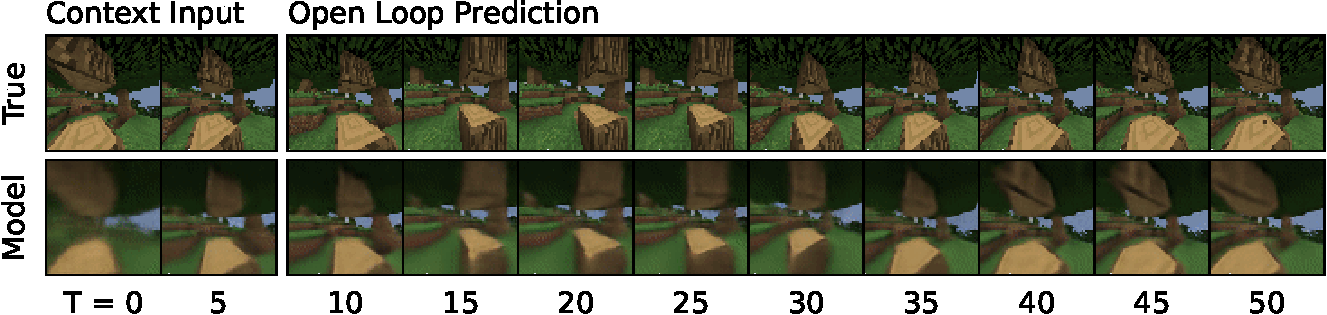
\includegraphics[width=\linewidth,trim={0 .5cm 0 .5cm},clip]{openl/mine4} \\[1ex]
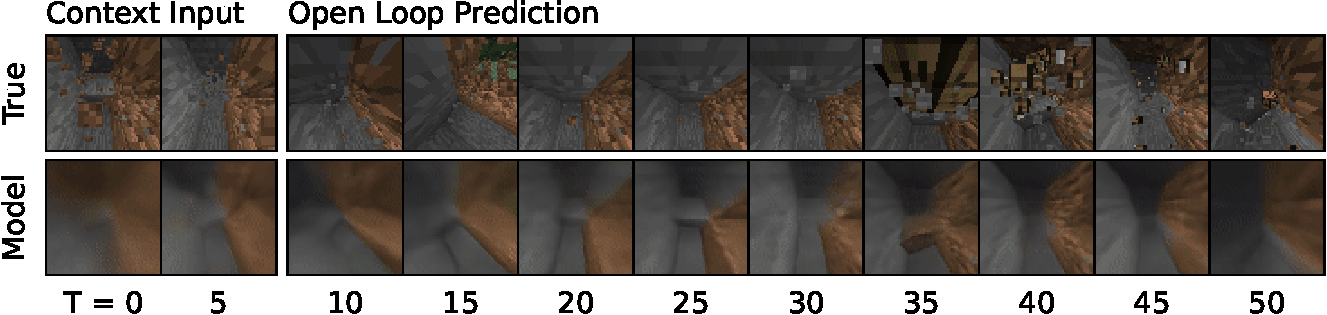
\includegraphics[width=\linewidth,trim={0 .5cm 0 .5cm},clip]{openl/mine5} \\[1ex]
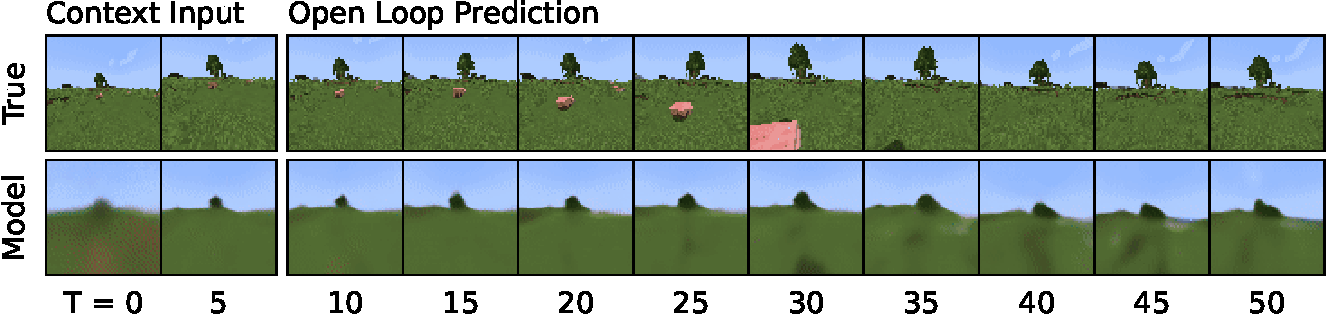
\includegraphics[width=\linewidth,trim={0 0 0 .5cm},clip]{openl/mine6} \\[1ex]
\caption{Multi-step predictions on Minecraft. The model receives the first 5 frames as context input and the predicts 45 steps into the future given the action sequence and without access to intermediate images.}
\label{fig:openl_more}
\end{figure}
